

\section{Data processing}

The following two sections will cover the implementation of the filter used to prepare the EMG-signal and the extraction of features to represent the signal. Choices behind implemented methods builds on background knowledge acquired in \secref{sec:pross}. 


\subsection{Filtering of signal} \label{sec:prePros} 

As earlier mentioned in \secref{sec:filt}, due to the MYB specifications limiting the sample rate to 200 Hz and movement artefact's in the low-frequency spectrum, it would be resourceful to implement a bandpass filter to avoid a biased signal.
In the interest of representing the signal with its true properties a second order Butterworth bandpass filter has been implemented with cut-off frequencies of 10 Hz and 90 Hz. A filter steeper than second order was deselected due to a chosen trade-off between filter performance and computational performance, which is of great importance when doing real-time control. Below in \figref{fig:filt} is the result of implementing the bandpass filter shown. The unfiltered signal (top) shows frequency components in low-frequency spectrum around 0-10 Hz and indicating frequency components above above 100 Hz. Both ends of the spectrum has been dampened limiting impact of artefact's and possible aliasing. Furthermore is the presence of the build-in 50 Hz notch filter elucidated as explained in \secref{sec:MYB}.     


\begin{figure}[H]                 
	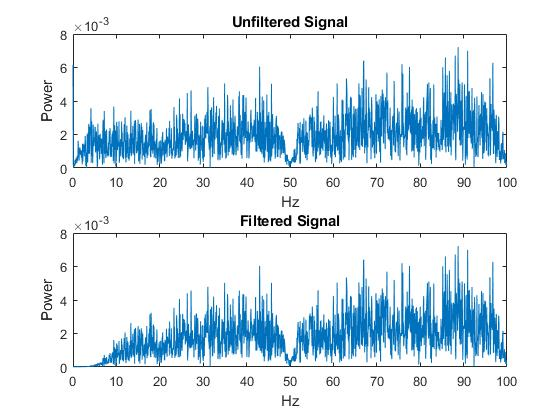
\includegraphics[width=.8\textwidth]{figures/pMethods/Filt}  
	\caption{Output showing the difference before an after implementing the bandpass filter. The unfiltered signal shows frequency components in low-frequency spectrum around 0-10 Hz and indicating frequency components above above 100 Hz. }
	\label{fig:filt} 
\end{figure}





\subsection{Feature extraction}

The features chosen to represent the information of movements contained in the signal is primarily based on recommendations from \cite{Donavan2017} where they found the optimal features for a real-time classification control scheme using the MYB. Donavan et al. used so called space domain features along with the MYB and got a five percent higher accuracy than by using the well known Hudgins time domain features. A total of seven features, Mean Absolute Value (MAV), Mean Mean Absolute Value (MMAV), Scaled Mean Absolute Value (SMAV), Correlation Coefficient (CC), Mean Absolute Difference Normalized (MADN), Mean Absolute Difference Raw (MADR) and Scaled Mean Absolute Difference Raw (SMADR) were derived and the following section will explain the extraction of each. Only SMAV, CC, MADN and SMADR were used for the final classification to reduce redundancy, but all seven will be explained because the some features are a combination of others. \cite{Donavan2017} Furthermore it has been chosen to extract the time domain feature of waveform length (WL) to represent frequency related information of the signal. The extraction of this feature will lastly be explained as well. 

\begin{flalign}
	MAV_i=\frac{\sum_{n=1}^{wl}}{wl}
	\label{TP}
\end{flalign}
      




\begin{flalign}
	MMAV=\frac{\sum_{i=1}^{8}MAV}{8}
	\label{TP}
\end{flalign}




\begin{flalign}
	SMAV_i=\frac{MAV_i}{MMAV}
	\label{TP}
\end{flalign}




\begin{flalign}
	CC_i=\frac{\sum_{n=1}^{wl}X_i[n]X_{i+1}[n]}{\sum_{n=1}^{wl}X_i[n]^2}=\frac{\sum_{n=1}^{wl}X_i[n]X_{i+1}[n]}{wl}
	\label{TP}
\end{flalign}



\begin{flalign}
	MADN_i=\frac{\sum_{n=1}^{wl}|X_i[n]-X_{i+1}[n]|}{\sum_{n=1}^{wl}X_i[n]^2}=\frac{\sum_{n=1}^{wl}|X_i[n]-X_{i+1}[n]|}{wl}
	\label{TP}
\end{flalign}


\begin{flalign}
	MADR_i=\frac{\sum_{n=1}^{wl}|X_i[n]-X_{i+1}[n]|}{wl}
	\label{TP}
\end{flalign}




\begin{flalign}
	SMADR_i=\frac{MADR_i}{MMAV}
	\label{TP}
\end{flalign}















